\documentclass[12pt]{article}
\usepackage[utf8]{inputenc}
\usepackage[T1]{fontenc}
\usepackage[english]{babel}
\usepackage{amsmath, amssymb, amsthm}
\usepackage{geometry}
\usepackage{titling}
\usepackage{fancyhdr}
\usepackage{lipsum}
\usepackage{parskip}
\usepackage{forest}
\usepackage{tikz}
\usepackage{stmaryrd}
\usepackage{listings}
\usepackage{graphicx}
\usepackage{float}
\usepackage{alphalph}
\usepackage{cancel}
\usepackage{textgreek}
\usepackage{titlesec}
\usepackage{dsfont}
\usepackage{caption}
\usepackage{listings}
\usepackage{subcaption} % for subfigures

\geometry{top=4cm, bottom=4cm, left=4cm, right=4cm}
\pagestyle{fancy}
\fancyhf{}
\rhead{Pierre Pili $\cdot$ Marie Gardie $\cdot$ Isée Biglietti}
\lhead{Econometrics 3}
\cfoot{\thepage}
\setlength{\headheight}{14.49998pt}
\addtolength{\topmargin}{-2.49998pt}

\titleformat{\section}{\small\bfseries}{\thesection}{1em}{}
\renewcommand{\thesubsection}{\arabic{section}.\arabic{subsection}}
\renewcommand{\thesubsubsection}{\arabic{section}.\arabic{subsection}.\alph{subsubsection}}

\title{Problem Set 7}
\author{PILI Pierre $\cdot$ GARDIE Marie $\cdot$ BIGLIETTI Isée}
\date{\today}

% Redéfinir le format de numérotation des sous-sections
\titleformat{\subsection}
  {\normalfont\small\bfseries}{\alph{subsection})}{1em}{}
  
\begin{document}
\maketitle
\renewcommand{\thesubsection}{\alph{subsection}}

\section{Show that, under the assumption of homogeneous treatment effects, Wooldridge’s Assumption $FE_1$ implies the parallel trends assumption does not vary with g (for any $t \geq 2$).}
We compute the last expression and will make use of the different assumptions along the way to derive an expression which does not depend on $g$. The homogeneity of the treatment and the linear model yields
\begin{align*}
    \mathbb{E}\left(Y_{g, t}(0) - Y_{g, t-1}(0)\right) &= \mathbb{E}\left(\alpha_g + \lambda_t + \beta \cdot  0 + \varepsilon_{g, t} - \alpha_g - \lambda_{t-1} - \beta \cdot 0 - \varepsilon_{g, t-1}\right) 
\end{align*}
which simplifies to
\begin{align*}
    \mathbb{E}\left(Y_{g, t}(0) - Y_{g, t-1}(0)\right) &= \mathbb{E}\left(\lambda_t - \lambda_{t-1}\right)  + \mathbb{E}\left(\varepsilon_{g, t} - \varepsilon_{g, t-1}\right) 
\end{align*}
The first term does not depend on $g$. The second is equal to zero, indeed, according to the law of iterated expectations,
$$\mathbb{E}\left(\varepsilon_{g, t}\right) = \mathbb{E}\big(\mathbb{E}(\varepsilon_{g, t}|\alpha_g, D_{g, t})\big) = 0$$
and similarly for $t-1$. We have proved the expected result.
\setcounter{section}{2}
\section{Coding part}
\subsection{Note that the treatment effect estimate for group 2007 and time 2004 is equal to the event study estimate for event time -3. Similarly, note that the treatment effect estimate for group 2004 and time 2007 is equal to the event study estimate for event time 3. Why is this so?}
The only group for which we can study a treatment effect three years before treatment is the 2007 group. Therefore the -3 parameter in the event study is identical as the treatment effect for group 2007 in 2004. The same goes for group 2004 in 2007, it is the only group for which we can evaluate a treatment effect three years after treatment.
\subsection{How many never treated groups (or counties) are there?}
Running a short piece of code and not forgetting to group by the $countyreal$ variable we get 309 never treated counties.
\subsection{Redo the analysis using the not yet treated group as control group. How do the results compare? Are you surprised (given your answer to the previous question)?}
At first glance the results seem very similar (see Figure \ref{fig:both_images}). (More analysis is welcomed)
\begin{figure}[htbp]
    \centering
    \begin{subfigure}[b]{0.9\textwidth}
        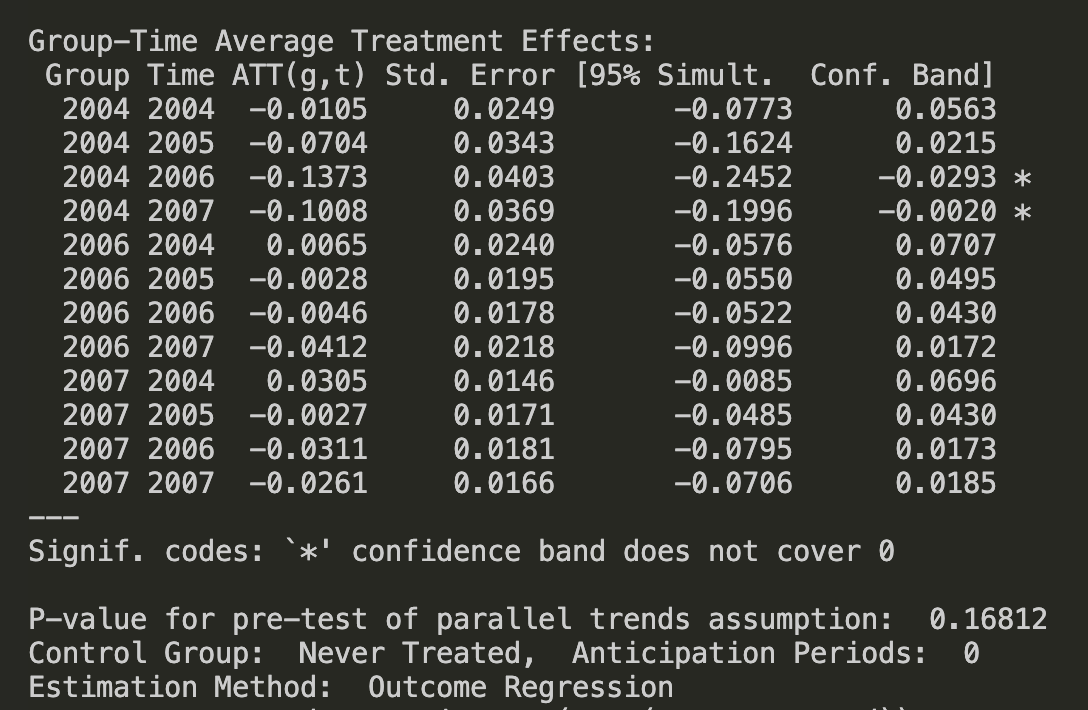
\includegraphics[width=\textwidth]{media/never_treated.png} % Include first image
        \caption{Never Treated Estimation}
        \label{fig:img1}
    \end{subfigure}
    \hfill
    \begin{subfigure}[b]{0.9\textwidth}
        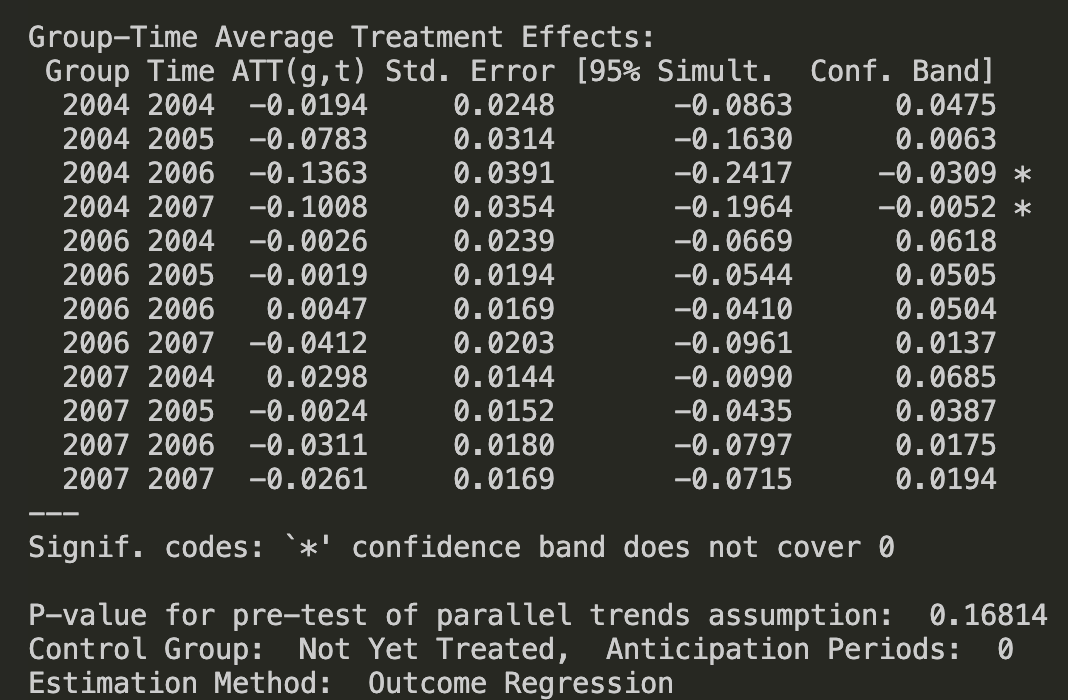
\includegraphics[width=\textwidth]{media/not_yet_treated.png} % Include second image
        \caption{Not Yet Treated}
        \label{fig:img2}
    \end{subfigure}
    \caption{Did Estimates}
    \label{fig:both_images}
\end{figure}
\subsection{Define the treatment variable D equal to 1 if county g is treated in time t and 0 otherwise, i.e., replace the “...” with the appropriate code in the ExampleDID.R file. Then use the two-way fixed effects estimator to estimate the treatment effect. What do you find? How does your estimate compare to the corresponding estimate(s) obtained using the “did” package?}

% Table created by stargazer v.5.2.3 by Marek Hlavac, Social Policy Institute. E-mail: marek.hlavac at gmail.com
% Date and time: Jeu, avr 04, 2024 - 15:45:11
\begin{table}[!htbp] \centering 
  \caption{Two-Way Fixed Effects Estimate} 
  \label{2wfe} 
\begin{tabular}{@{\extracolsep{5pt}}lc} 
\\[-1.8ex]\hline 
\hline \\[-1.8ex] 
 & \multicolumn{1}{c}{\textit{Dependent variable:}} \\ 
\cline{2-2} 
\\[-1.8ex] & lemp \\ 
\hline \\[-1.8ex] 
 D & $-$0.296$^{***}$ \\ 
  & (0.072) \\ 
  & \\ 
\hline \\[-1.8ex] 
Observations & 2,500 \\ 
R$^{2}$ & 0.007 \\ 
Adjusted R$^{2}$ & 0.005 \\ 
F Statistic & 17.019$^{***}$ (df = 1; 2494) \\ 
\hline 
\hline \\[-1.8ex] 
\textit{Note:}  & \multicolumn{1}{r}{$^{*}$p$<$0.1; $^{**}$p$<$0.05; $^{***}$p$<$0.01} \\ 
\end{tabular} 
\end{table} 

By using the plm package we estimated the two-way fixed effects estimator (see Table \ref{2wfe})
\subsection{Implement the “classical” event study design using the two-way fixed effects estimator. What do you find? How do your estimates compare to the (sets of) estimates obtained using the “did” package?}
\subsection{Run the twowayfeweights function. What do you find?}
\begin{figure}[htbp]
    \centering
    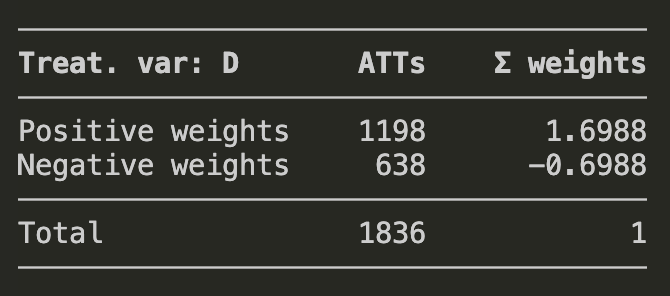
\includegraphics[width=0.7\textwidth]{media/2wfeg.png}
        \caption{twowayfeweights}
        \label{2wfew}
\end{figure}
\subsection{How do you interpret your findings in (d) and (f)?}
\end{document}
